\subsection{Taylor-Green vortex}
The Taylor-Green vortex problem is used to examine if our N-S code has the ability to correctly simulate vortex decay and turbulence \cite{DeBonis2013}. TGV is a non-trivial analytical  solution to N-S. We will compute and compare the kinetic energy dissipation rate against a well known very good solver (smisk smisk). This will help us determine the solvers ability to handle turbulence. 
\subsubsection{Problem definition}
Using a cube with sides $2\pi$. \newline
We have an initial distribution of velocity $\bar{u} = (u,v,w)$:
\begin{align}
u(x,y,z) &= V_0sin(x)cos(y)cos(z) \\
v(x,y,z) &= - V_0cos(x)sin(y)cos(z)  \\
w(x,y,z) &= 0  
\end{align}
The Reynolds number is defined as: $Re = \frac{V_0 L}{\nu}$ where we set $V_0 = 1$

\subsubsection*{Something about calculating data}
The method used to evaluate the TGV solutions will be by investigating the rate of which the fluid dissipates the kinetic energi. The kinetic energi will be calculated as:
$$        E_k = \frac{1}{\rho_0 \Omega}\int \rho \frac{uu}{2} = 0.5 \frac{u^2}{(2pi)^3}$$
We use this to calculated the dissipation rate by differentiating $E_k$ w.r.t time:
$$ \epsilon(E_k) = -\frac{d E_k}{dt}$$

\subsubsection*{Results}
To help validate the Taylor-Green solutions we used the Oasis solver \cite{Oasis} which is known to handle TGV and other turbulent flows. We look at a plot of the dissipation rate over time and the kinetic energi compared with Oasis. 
These test were run with: N = 32, $\Delta t = 0.001$ , $\nu = 0.001$ giving Re = 1000:

\begin{center}
\begin{figure}[h!]
\centering
\begin{minipage}{.5\textwidth}
  \centering
  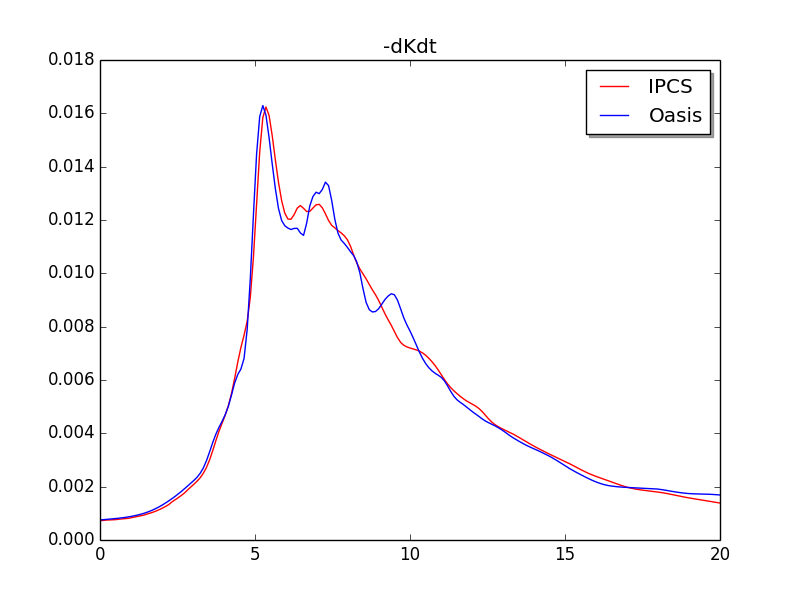
\includegraphics[scale=0.4]{./Verification_Validation/TaylorGreen/Dkdt.png}
  \captionof{figure}{$\epsilon(E_k)$ N = 32}
  \label{fig:test1}
\end{minipage}%
\begin{minipage}{.5\textwidth}
  \centering
  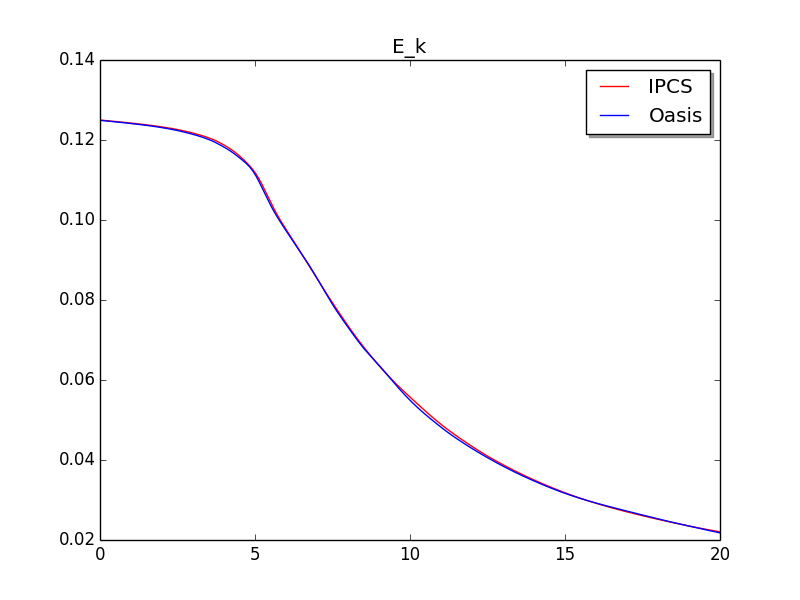
\includegraphics[scale=0.4]{./Verification_Validation/TaylorGreen/Ek.png}
  \captionof{figure}{$E_k$ N = 32 }
  \label{fig:test2}
\end{minipage}
\end{figure}
\end{center}
































